\documentclass[noinstructornotes]{ximera}
%handout:  for handout version with no solutions or instructor notes
%handout,instructornotes:  for instructor version with just problems and notes, no solutions
%noinstructornotes:  shows only problem and solutions

%% handout
%% space
%% newpage
%% numbers
%% nooutcomes

%I added the commands here so that I would't have to keep looking them up
%\newcommand{\RR}{\mathbb R}
%\renewcommand{\d}{\,d}
%\newcommand{\dd}[2][]{\frac{d #1}{d #2}}
%\renewcommand{\l}{\ell}
%\newcommand{\ddx}{\frac{d}{dx}}
%\everymath{\displaystyle}
%\newcommand{\dfn}{\textbf}
%\newcommand{\eval}[1]{\bigg[ #1 \bigg]}

%\begin{image}
%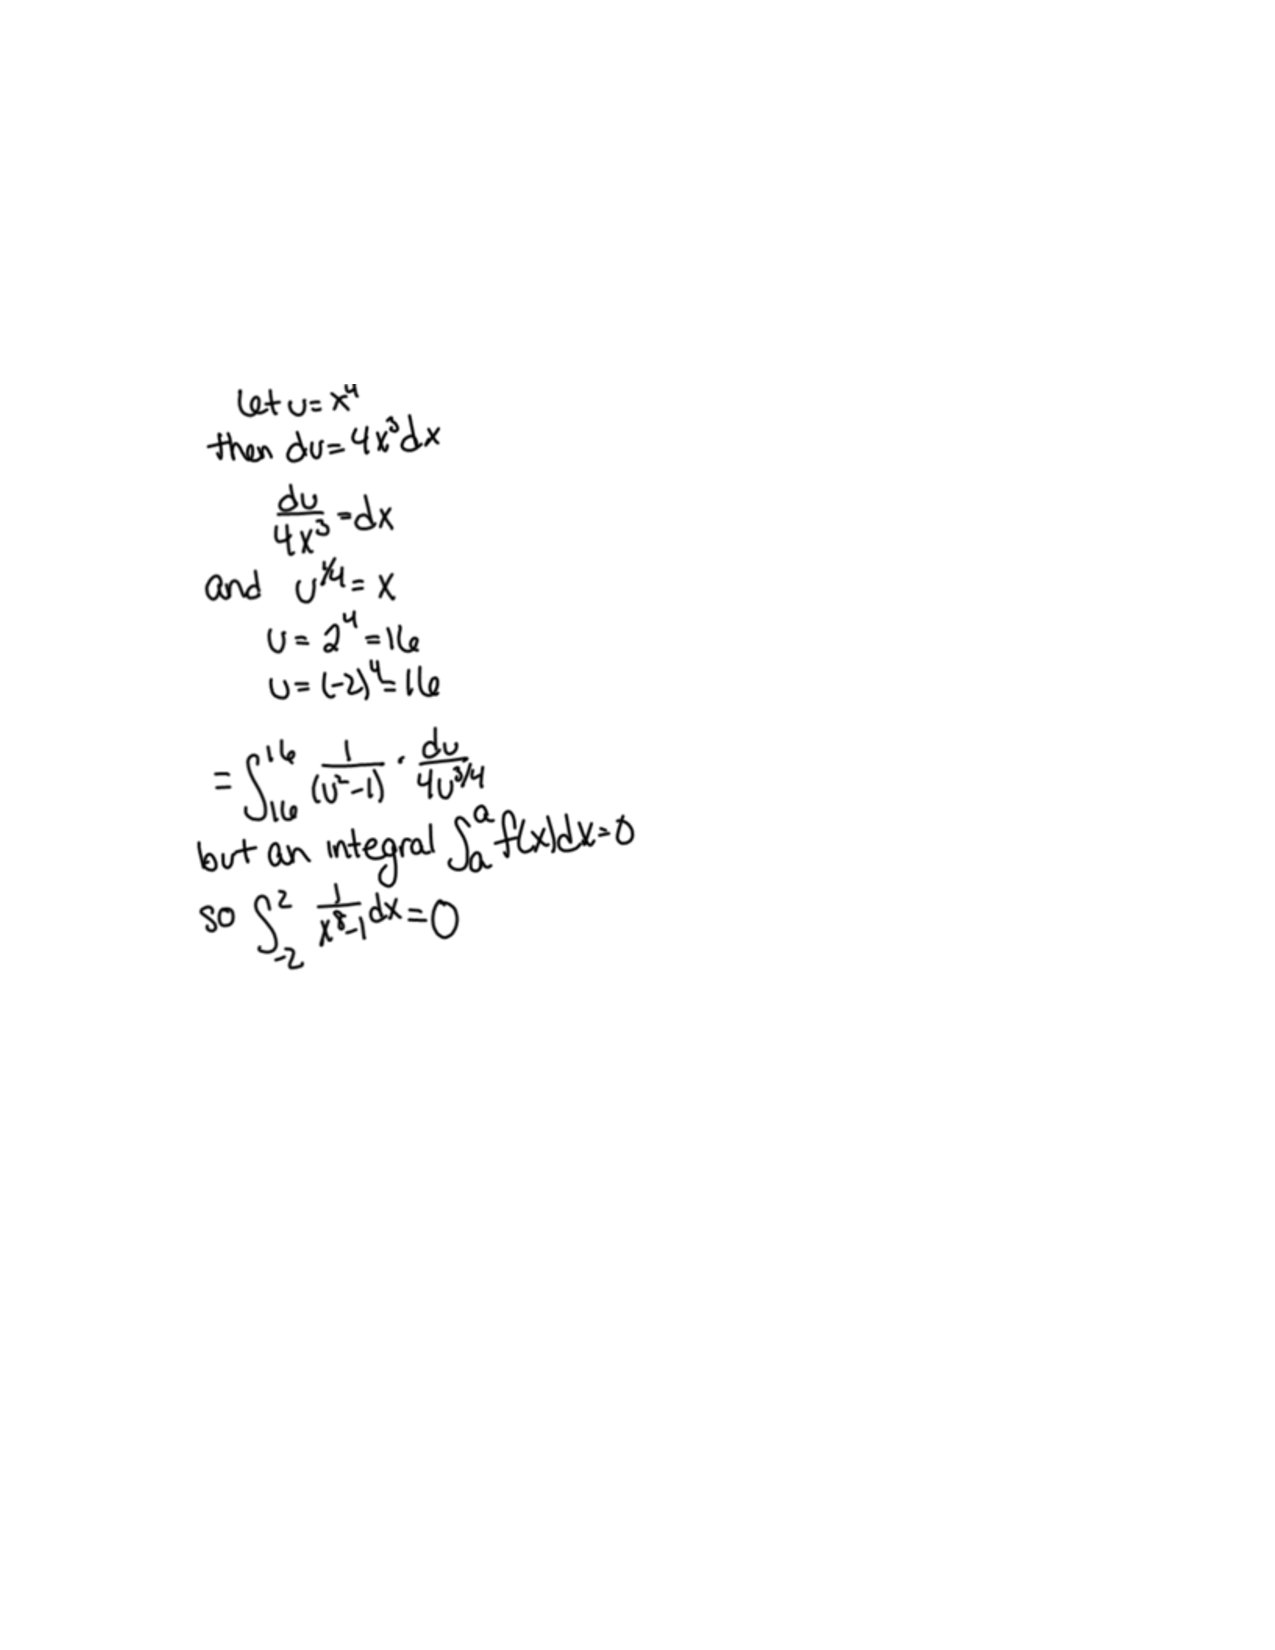
\includegraphics[trim= 170 420 250 180]{Figure1.pdf}
%\end{image}

%add a ``.'' below when used in a specific directory.
\newcommand{\RR}{\mathbb R}
\renewcommand{\d}{\,d}
\newcommand{\dd}[2][]{\frac{d #1}{d #2}}
\renewcommand{\l}{\ell}
\newcommand{\ddx}{\frac{d}{dx}}
\newcommand{\dfn}{\textbf}
\newcommand{\eval}[1]{\bigg[ #1 \bigg]}

\usepackage{multicol}

\renewenvironment{freeResponse}{
\ifhandout\setbox0\vbox\bgroup\else
\begin{trivlist}\item[\hskip \labelsep\bfseries Solution:\hspace{2ex}]
\fi}
{\ifhandout\egroup\else
\end{trivlist}
\fi} %% we can turn off input when making a master document
\usepackage{fullpage}

\title{Recitation \#17: The Ratio, Root, Comparison, and Limit Comparison Tests}  

\begin{document}
\begin{abstract}		\end{abstract}
\maketitle












\section{Group work:}

%Comparison Test Problem
\section{Warm up:}
For each of the following, answer {\bf True} or {\bf False}, and explain why.
	\begin{enumerate}
	
	\item  If $a_n \geq 0$ and $\sum_{n=0}^\infty a_n$ converges, then $\sum_{n=0}^\infty a_n^2$ converges.
	
	\item  If $a_n, b_n \geq 0$ and both $\sum_{n=0}^\infty a_n$ and $\sum_{n=0}^\infty b_n$ converge, then $\sum_{n=0}^\infty a_n b_n$ converges. 
	
	\end{enumerate}
	
	\begin{freeResponse}
		\begin{enumerate}
		
		\item  \dfn{True}
		
		Since $\sum_{n=0}^\infty a_n$ converges, $\lim_{n \to \infty} a_n = 0$.  
		So, in particular, there exists an integer $N$ such that $a_k < 1$ for all $k \geq N$.  
		Then for all $k \geq N$, $a_k^2 < a_k$, and therefore we have that
			\[
			\sum_{n=N}^\infty a_n^2 < \sum_{n=N}^\infty a_n.
			\]
		Thus,  by the Comparison Test, $\sum_{n=0}^\infty a_n^2$ is convergent.
		
		
		
		\item  \dfn{True}
		
		Just as in part (a) there exists an integer $N$ such that $a_k < 1$ for all $k \geq N$.  
		Then
			\[
			\sum_{n=N}^\infty a_n b_n < \sum_{n=N}^\infty b_n
			\]
		and thus, by the Comparison Test, $\sum_{n=0}^\infty a_n b_n$ is convergent.
		
		\end{enumerate}
	\end{freeResponse}
	
\begin{instructorNotes}
Show that these series converge formally using the comparison test.
\end{instructorNotes}







\section{Group work:}



%problem 1
\begin{problem}
	\begin{enumerate}
	
	\item  Why can we not use the Comparison test with $\sum_{k=1}^\infty \frac{1}{k^2}$ to show that $\sum_{k=1}^\infty \frac{1}{k^2 - 5}$ converges?
	
	\item  Adjust $\sum_{k=1}^\infty \frac{1}{k^2}$ to show that $\sum_{k=1}^\infty \frac{1}{k^2 - 5}$ converges via the Comparison Test.
	
	\item  Give a convergent series we can use in the Limit Comparison Test to show that $\sum_{k=1}^\infty \frac{1}{k^2 - 5}$ converges.  
	
	\end{enumerate}
	
	\begin{freeResponse}
		\begin{enumerate}
		
		\item  We cannot use the Comparison Test here because 
			\[
			\frac{1}{k^2} < \frac{1}{k^2 - 5}
			\]
		for all $k \geq 1$.  So we would just be showing the the series in question is greater than a series which converges, which does not give us any information.
		
		
		
		\item  Notice that
			\[
			\frac{2}{k^2} > \frac{1}{k^2 - 5}
			\]
		for all $k \geq 4$.  
		Since $\sum_{k=1}^\infty \frac{1}{k^2}$ converges, $\sum_{k=1}^\infty \frac{2}{k^2} = 2 \sum_{k=1}^\infty \frac{1}{k^2}$.  
		Thus, $\sum_{k=1}^\infty \frac{2}{k^2}$ converges.
		
		Therefore, the Comparison Test with $\sum_{k=1}^\infty \frac{2}{k^2}$ shows that $\sum_{k=0}^\infty \frac{1}{k^2-5}$ converges.
		
		
		
		\item  For the Limit Comparison Test, we \dfn{can} use $\sum_{k=1}^\infty \frac{1}{k^2}$.  
			\begin{align*}
			\lim_{k \to \infty} \frac{\frac{1}{k^2-5}}{\frac{1}{k^2}}
			&= \lim_{k \to \infty} \frac{k^2}{k^2-5}  \\
			&= 1.
			\end{align*}
			
		Thus, since $\sum_{k=1}^\infty \frac{1}{k^2}$ converges, by the Limit Comparison Test we know that $\sum_{k=0}^\infty \frac{1}{k^2-5}$ converges.
		
		\end{enumerate}
	\end{freeResponse}

\end{problem}

\begin{instructorNotes}
This problem may be done as a quick whole class discussion.  
For (b), use something like $\frac{2}{k^2}$.  
Be sure to determine for which $k$ the inequality will hold.
\end{instructorNotes}







%Root and Ratio Test Problem
%problem 1
\begin{problem}
Determine if the following series converge or diverge.
	\begin{enumerate}
	
	\item  $\sum_{n=1}^\infty \frac{(7n+1)^2 \cdot 2^n}{5^n}$
	
	
	\item $\sum_{k=1}^{\infty} \frac{(k!)^3}{(3k)!}$
	
	\item  $\sum_{n=0}^\infty \frac{n^2 + 2n + 1}{3n^3+1}$
	
	\item  $\sum_{n=0}^\infty \frac{\cos^2 n}{n^3+1}$
	
	
	\end{enumerate}
	
	\begin{freeResponse}
		\begin{enumerate}
	
		\item  \dfn{Ratio Test}
			\begin{align*}
			\lim_{n \to \infty} \frac{a_{n+1}}{a_n} 
			&= \lim_{n \to \infty} \left[ \frac{(7(n+1) + 1)^2 \cdot 2^{n+1}}{5^{n+1}} \cdot \frac{5^n}{(7n+1)^2 \cdot 2^n} \right]  \\
			&= \lim_{n \to \infty} \frac{(7n+8)^2 \cdot 2}{5 \cdot (7n+1)^2}  \\
			&= \frac{49 \cdot 2}{49 \cdot 5} = \frac{2}{5}.
			\end{align*}
		Thus, since $\lim_{n \to \infty} \frac{a_{n+1}}{a_n} < 1$, this series \boxed{converges}.  
	

		\item \dfn{Ratio Test}
		\begin{align*}
			\lim_{k \to \infty} \frac{a_{k+1}}{a_k} 
			&= \lim_{k \to \infty} \left[ \frac{( (k+1)!)^3}{(3(k+1))!}  \cdot \frac{(3k)!}{(k!)^3} \right]  \\
			&= \lim_{k \to \infty} \frac{ (k+1)^3 (k!)^3}{(3k+3)(3k+2)(3k+1) \cdot (3k)!} \cdot \frac{(3k)!}{(k!)^3} \\
			&= \lim_{k \to \infty} \frac{(k+1)^3}{(3k+3)(3k+2)(3k+1)}  \\
			&= \frac{1}{3 \cdot 3 \cdot 3}= \frac{1}{27}.
			\end{align*}
		Thus, since $\lim_{k \to \infty} \frac{a_{k+1}}{a_k} < 1$, this series \boxed{converges}. 
		
			
			\item  Use the \dfn{Limit Comparison Test} with $\sum_{n=1}^\infty \frac{1}{n}$.
			\begin{align*}
			\lim_{n \to \infty} \frac{a_n}{b_n}
			&= \lim_{n \to \infty} \frac{n^2+2n+1}{3n^3+1} \cdot \frac{n}{1}  \\
			&= \frac{1}{3}.
			\end{align*}
			
		Therefore, since $\sum_{n=1}^\infty \frac{1}{n}$ diverges, by the Limit Comparison Test we know that $\sum_{n=0}^\infty \frac{n^2+2n+1}{3n^3+1}$ diverges.
		
		\item  Use the \dfn{Comparison Test} with $\sum_{n=1}^\infty \frac{1}{n^3}$.  
		
		Since we always have that $0 < \cos^2(n) < 1$, we know that
			\[
			\frac{\cos^2(n)}{n^3 + 1} \leq \frac{1}{n^3+1} < \frac{1}{n^3}.
			\]
		Therefore, by the Comparison Test, we have that $\sum_{n=0}^\infty \frac{\cos^2 n}{n^3+1}$ converges.
		
	
		
		
		\end{enumerate}
	\end{freeResponse}
	
\end{problem}

\begin{instructorNotes}
Let the students experiment with what tests to use.  
Perhaps give two problems per group.
\end{instructorNotes}










	
	
	
	
	
	
	
	
	

	










								
				
				
	














\end{document} 


















